% Okay, the general idea is as follows:
% I want to have have a group of bar plots showing a subset of my implementations vs. PWM, and Kaneta's extrapolated numbers however, it begs the question
% Which of my implementations do I choose?
% I want:
%
% - my fastest LUT variant 
% - my fastest <= 64 bit pext variant
% - 64 bit pshufb
% - 128, 256 and 512 bit pshufb/vpermb/vpcompressb
%
% The first three are to compare Kaneta's methods with the LUT method, the latter are for showing the performance increase with SIMD
% However, how do I know which of my pext and LUT variants are fastest? While I might know intuitively, I first have to show
% which of my LUT variants is fastest, and which of my pext variants is fastest.
% 
% This series of plots shows which LUT variant is fastest
%
% I don't wanna include every single text, since that would be seriously overkill, even though I might
% I feel PCC already offers a decent seleciton of texts

\documentclass[a4]{article}

\usepackage[utf8]{inputenc}
\usepackage[english]{babel}

\usepackage{amsmath,amsfonts,amssymb}
\usepackage{fullpage}
\usepackage{verbatim}

\usepackage{tikz,pgfplots}
\usetikzlibrary{patterns, patterns.meta}
\usepgfplotslibrary{groupplots}

\pgfplotsset{
    width = 150mm,
    height = 100mm,
    major grid style = { thin, dotted, color = black!50 },
    minor grid style = { thin, dotted, color = black!50 },
    grid,
    xtick distance = 1,
    ymin = 0,
    legend cell align = left,
    legend pos = north west,
	  /pgfplots/ybar legend/.style = {
		  /pgfplots/legend image code/.code={%
			  \draw[##1,/tikz/.cd,yshift=-0.35em]
      (0cm,0cm) rectangle (0.7em,0.8em);},
	  },  
}

\begin{document}

\title{WT Benchmark}
\author{Jan-Philipp Tarnowski}
\maketitle

\clearpage


% IMPORT-DATA stats ../results-pcc-regular.out

% SQL UPDATE stats SET file = 'dblp.xml' WHERE file LIKE '%dblp.xml'
% SQL UPDATE stats SET file = 'dna' WHERE file LIKE '%dna'
% SQL UPDATE stats SET file = 'english' WHERE file LIKE '%english'
% SQL UPDATE stats SET file = 'pitches' WHERE file LIKE '%pitches'
% SQL UPDATE stats SET file = 'proteins' WHERE file LIKE '%proteins'
% SQL UPDATE stats SET file = 'sources' WHERE file LIKE '%sources'


\begin{center}
    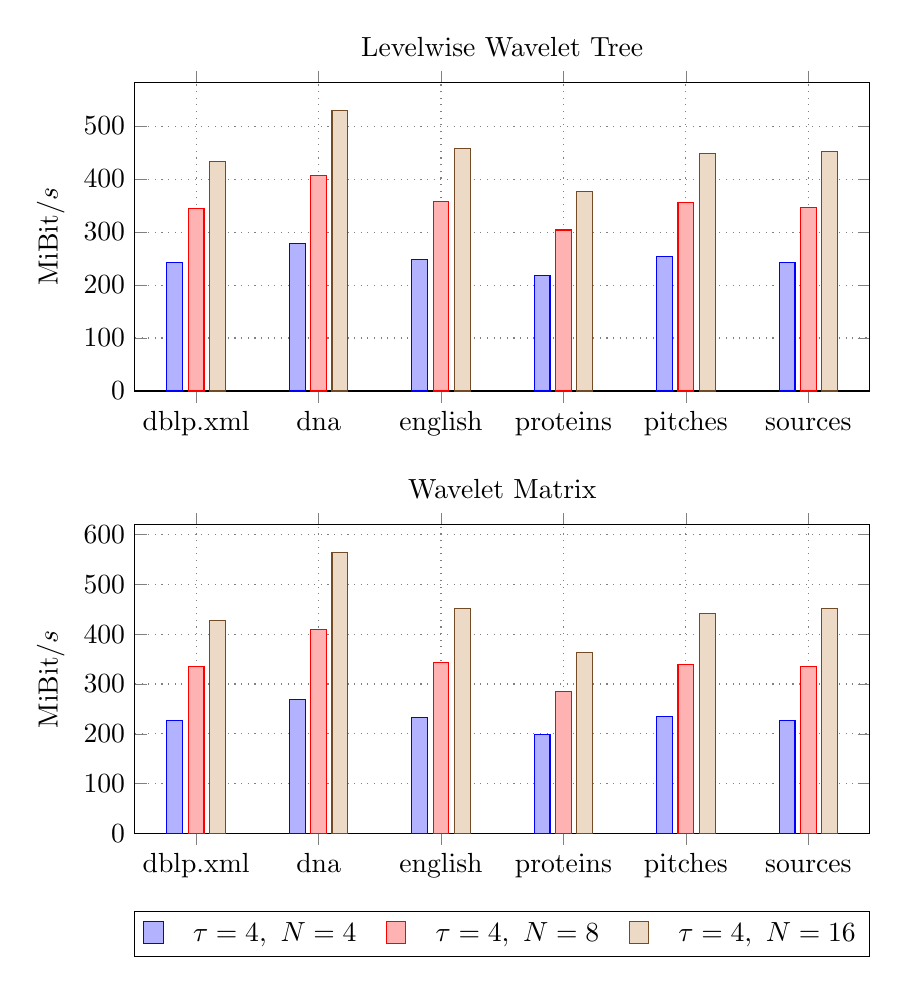
\begin{tikzpicture}
        \begin{groupplot} [
            width = 0.9\textwidth,
            height = 5.5cm,
            xticklabel style = {
                text height = 1.5ex
            },
            ybar,
            group style = { 
                vertical sep = 1.7cm,
                group size = { 
                    1 by 2
                } 
            },
            symbolic x coords = {
                dblp.xml,
                dna,
                english,
                proteins,
                pitches,
                sources
            },
            ylabel = $\text{MiBit}/s$,
            legend style = { 
                at = {(0.5, -0.25)},
                anchor = north,
                legend columns = -1,
                column sep = 2ex
            },
            ytick distance = 100,
        ]
        
        
        \nextgroupplot [
            title = Levelwise Wavelet Tree,
            bar width = 0.2cm,
        ]

			%% MULTIPLOT(type) SELECT file AS x, MEDIAN((height * (size / CAST(time_in_s AS Float))) / (1024 * 1024)) AS y,MULTIPLOT
			%% FROM stats WHERE type LIKE 'lwt_lut_%' GROUP BY MULTIPLOT,x ORDER BY ds_order,MULTIPLOT,x
   \addplot coordinates { (dblp.xml,242.51) (dna,279.132) (english,248.163) (pitches,253.08) (proteins,217.555) (sources,243.198) };
   \addlegendentry{type=lwt\_lut\_4\_4\_1};
   \addplot coordinates { (dblp.xml,344.077) (dna,406.921) (english,356.868) (pitches,355.53) (proteins,303.895) (sources,347.179) };
   \addlegendentry{type=lwt\_lut\_8\_4\_2};
   \addplot coordinates { (dblp.xml,433.435) (dna,529.317) (english,456.909) (pitches,448.023) (proteins,375.731) (sources,451.243) };
   \addlegendentry{type=lwt\_lut\_16\_4\_4};

   \legend{};


   \nextgroupplot [
    title = Wavelet Matrix,
    bar width = 0.2cm
]

   %% MULTIPLOT(type) SELECT file AS x, MEDIAN((height * (size / CAST(time_in_s AS Float))) / (1024 * 1024)) AS y,MULTIPLOT
   %% FROM stats WHERE type LIKE 'wm_lut_%' GROUP BY MULTIPLOT,x ORDER BY ds_order,MULTIPLOT,x
   \addplot coordinates { (dblp.xml,227.59) (dna,268.419) (english,233.415) (pitches,235.517) (proteins,199.536) (sources,227.265) };
   \addlegendentry{type=wm\_lut\_4\_4\_1};
   \addplot coordinates { (dblp.xml,335.441) (dna,409.362) (english,343.009) (pitches,340.01) (proteins,285.607) (sources,335.973) };
   \addlegendentry{type=wm\_lut\_8\_4\_2};
   \addplot coordinates { (dblp.xml,426.991) (dna,563.284) (english,451.729) (pitches,441.517) (proteins,363.248) (sources,451.855) };
   \addlegendentry{type=wm\_lut\_16\_4\_4};

   \legend{
          $\tau = 4,\ N = 4$\\
          $\tau = 4,\ N = 8$\\
          $\tau = 4,\ N = 16$\\
   }


        \end{groupplot}
    \end{tikzpicture}
\end{center}

\end{document}
